\section{QGP in small systems}

\begin{figure}[thb]
  \begin{center}
    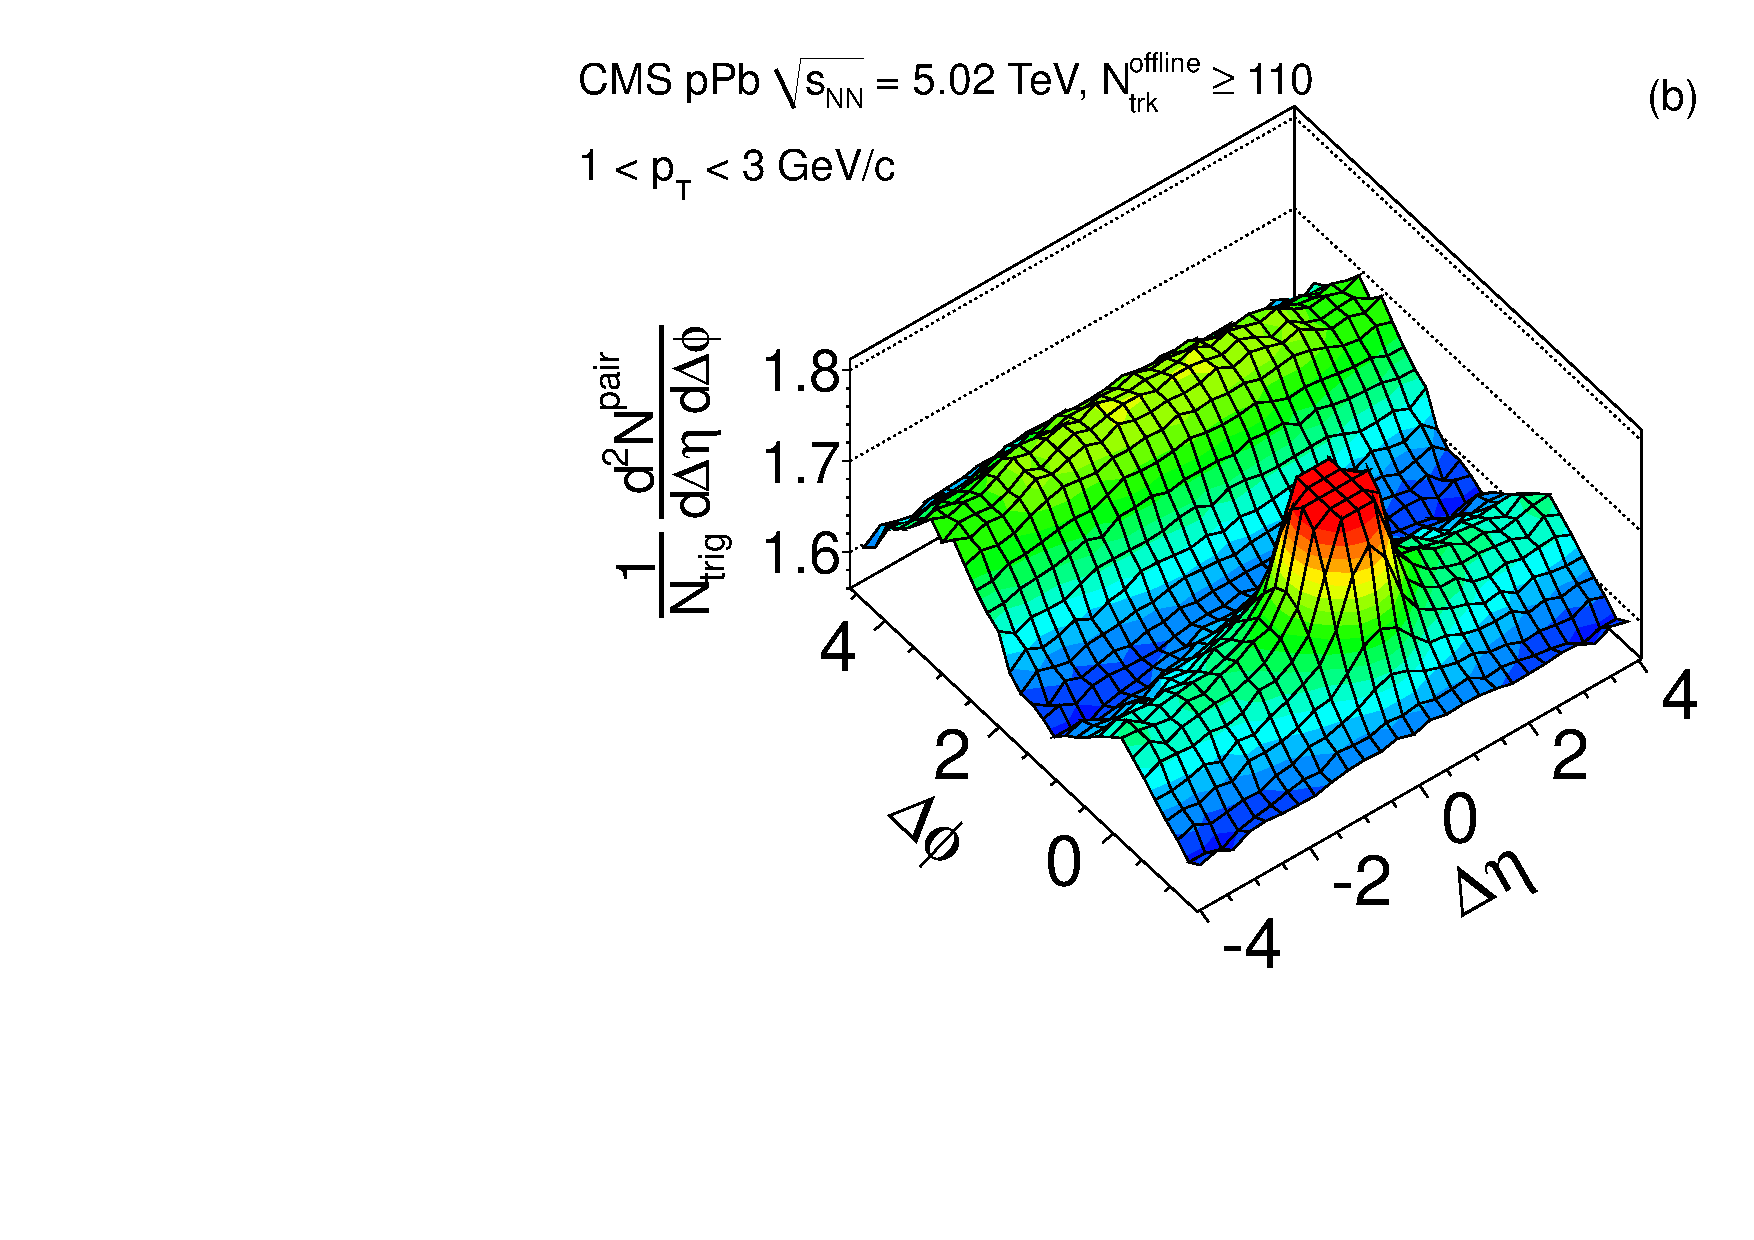
\includegraphics[width=0.4\textwidth]{figures/corr2D_pPb_N110_pt1-3_20121016.pdf}
    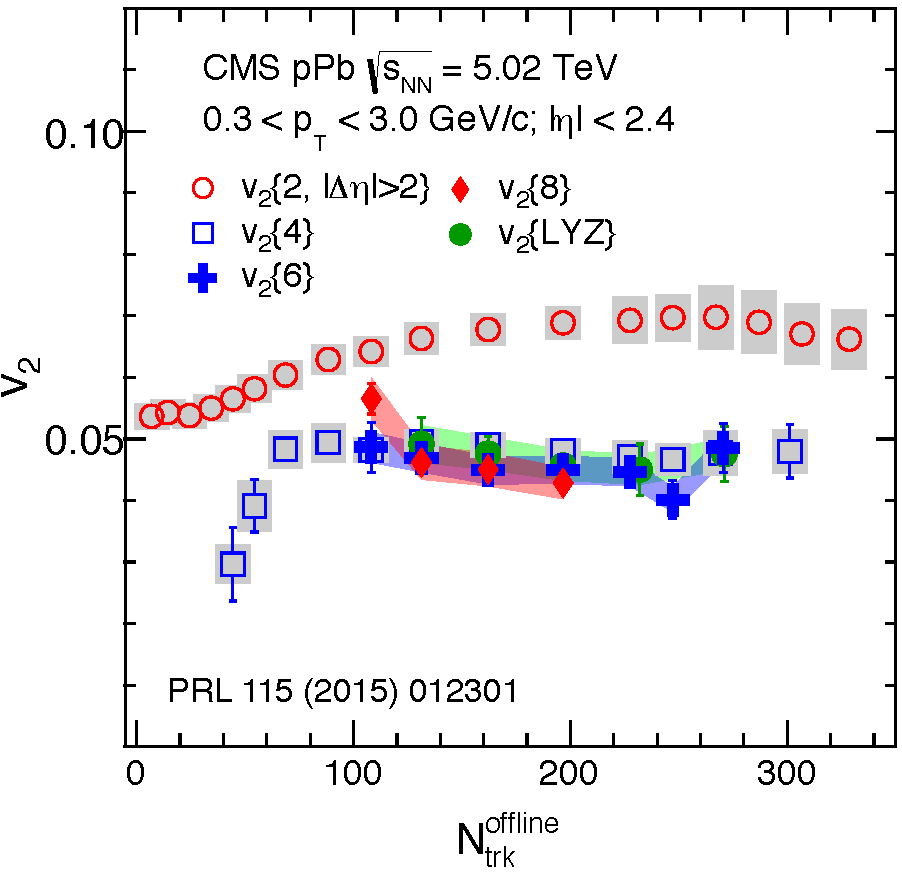
\includegraphics[width=0.4\textwidth]{figures/v2m_pPb.pdf}
    \caption{ Left: The 2D two-particle correlation functions in high-multiplicity 
    pPb collisions at \rootsNN\ = 5.02 TeV measured by the CMS experiment.
    Right: The elliptic anisotropy, $v_2$, as a function of $N_{\rm trk}$
    obtained from two-, four-, six- and eight-particle cumulants, and the LYZ method, 
    averaged over $0.3<\pt<3.0$~GeV/c, in pPb collisions at \rootsNN\ = 5.02 TeV.
  %~\cite{Khachatryan:2015waa}.
    }
    \label{fig:ridge_pPb}
  \end{center}
\end{figure} 

Observation of a long-range, near-side structure (often called ``Ridge'') in two-particle
\deta\ -- \dphi\ correlation function of high-multiplicity pp and pPb collisions, shown in Fig.~\ref{fig:ridge_pPb} 
(left), at CMS opened up new opportunities for studying novel dynamics of particle production 
in small but high-density Quantum Chromodynamic (QCD) systems. Similar ridge-like structure is
first observed in relativistic nucleus-nucleus (AA) collisions, and is attributed to the 
hydrodynamic collective flow of a strongly interacting and expanding medium. 

The origin of the ridge correlation structure in small colliding systems like pp and pPb
has not been conclusive yet in the community. While the formation of a hot and dense fluid-like
medium provides a natural explanation, it was not expected because the overlapping region 
is significantly smaller than that in an AA collision. Various alternative theoretical interpretations
have been proposed, such as initial-state gluon correlations without any final-state interactions.

A key observation made by CMS in 2013 pPb run at \rootsNN\ = 5.02 TeV is that
the elliptic azimuthal anisotropy harnomics, $v_2$, extracted using four-, six-,
eight- and all particle azimuthal correlations, are found to be nearly identically
within about 10\%, lending strong support to the highly collective nature of correlations 
in these systems. 

While much progress has been made in run 1, a lot of questions still remain unanswered: (1)
What is the origin of the observed collectivity? Is it a consequence of strong final-state
rescatterings in an initially eccentric system (like AA collisions)? Or it is rooted
in the initial momentum space due to initial-state gluon interactions? (2) If a hot and opaque 
medium is indeed formed in a pPb collision, how does it influence the behavior of hard probes
such as jets and quarkonia? Higher energy and luminosity pPb collisions at the LHC run 2 
will enable a wide range of high precision measurements, providing unique opportunities 
of addressing these important questions. 